%
% einfall.tex
%
% (c) 2018 Prof Dr Andreas Müller, Hochschule Rapperswil
%
\documentclass[tikz]{standalone}
\usepackage{times}
\usepackage{amsmath}
\usepackage{txfonts}
\usepackage[utf8]{inputenc}
\usepackage{graphics}
\usetikzlibrary{arrows,intersections}
\begin{document}
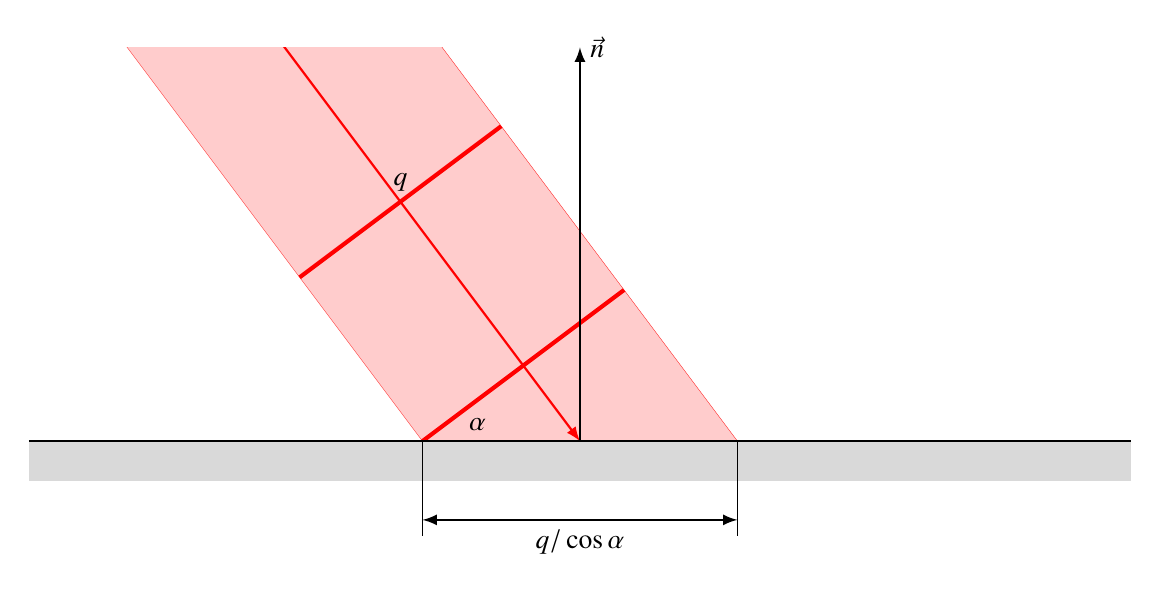
\begin{tikzpicture}[thick, >= latex, scale=1]

\begin{scope}
\clip (-6,0) rectangle (6,5);
\fill[color=red!20] ({-6-2},{8})--({3-2},{-4})--({3+2},-4)--({-6+2},8)--cycle;
\draw[line width=0.1,color=red] ({-6-2},{8})--({3-2},{-4});
\draw[line width=0.1,color=red] ({3+2},-4)--({-6+2},8);
\draw[->,color=red] (-6,8)--(0,0);
\end{scope}

\def\q{16/5}
\draw[color=red,line width=1.5pt] (-1,4)--({-1-\q*4/5},{4-\q*3/5});
\node at ({-1-0.5*\q*4/5},{4-0.5*\q*3/5}) [above] {$q$};

\draw[color=red,line width=1.5pt] (-2,0)--({-2+\q*4/5},{+\q*3/5});
\node at ({-2+0.7},0) [above] {$\alpha$};

\fill[color=gray!30] (-7,0)--(7,0)--(7,-0.5)--(-7,-0.5)--cycle;
\draw (-7,0)--(7,0);
\draw[->] (0,0)--(0,5) coordinate[label={right:$\vec n$}];

\draw[line width=0.1pt] (-2,0)--(-2,-1.2);
\draw[line width=0.1pt] (2,0)--(2,-1.2);
\draw[<->] (-2,-1)--(2,-1);
\node at (0,-1) [below] {$q/\cos\alpha$};

\end{tikzpicture}
\end{document}

